\documentclass[12pt]{article}
\usepackage{graphicx}          % Support for including images
\graphicspath{ {./images/} }
\usepackage{fontspec}  % Required for font selection with XeLaTeX/LuaLaTeX
\usepackage{blindtext}
\usepackage{tikz}
\usepackage{multicol}
\usepackage[most]{tcolorbox}
\usepackage{xcolor}
\usepackage{setspace}
\usepackage[top=0cm, left=0cm,right=1.5cm,bottom=0cm]{geometry}
\usepackage{ragged2e}
\usepackage[colorlinks=true, linkcolor=links, urlcolor=links, pdfborder={0 0 0}, pdfhighlight=/N]{hyperref}
\usepackage{enumitem}
\usepackage{lipsum}
\usepackage{paracol}
\usepackage{changepage}
\setmainfont{Times New Roman}
\definecolor{bgcolor}{HTML}{203864}
\definecolor{textcolor}{HTML}{303030}
\definecolor{links}{HTML}{2660c7}
%Strongly discourage hyphenation
\hyphenpenalty=10000
\exhyphenpenalty=10000
% Left align text
\RaggedRight
\color{textcolor}

\title{Giorgos Paphitis}
\author{Giorgos Paphitis}

\begin{document}
\pagestyle{empty}
\columnratio{0.30,0.50}
\begin{paracol}{2} % sync off, 2 columns
   \setlength{\columnsep}{12pt} % space between columns

   % LEFT COLUMN
   \begin{tcolorbox}[colback=bgcolor, colframe=bgcolor, boxrule=0cm, arc=0cm, outer arc=0cm, left=0.35cm, right=0.10cm, top=1cm, bottom=1.5cm,height=\textheight]
      \setlength{\leftskip}{5pt}
      \setlength{\rightskip}{5pt}
      \begin{center}
         \begin{tikzpicture}
            \def\radius{2.1cm}
            \draw[line width=4pt, color=white] (0,0) circle (\radius);
            \clip (0,0) circle (\radius);
            \node at (0,0) {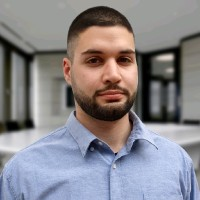
\includegraphics[scale=0.6]{giorgos_paphitis}};
         \end{tikzpicture}
      \end{center}
      \color{white}
      % ^ ABOUT ME
      \vspace{0.6cm}
      {\fontsize{12pt}{18pt}\selectfont
         \textbf{{\large About me}}\\
         }
      \vspace{0.15cm}
      \hrule
      \vspace{0.2cm}
      {\fontsize{10pt}{18pt}\selectfont
         I am a driven individual that always strives to succeed in all aspects of my life. This characteristic has helped me achieve goals like, highest grade in the 2021 Pancyprian Computer Science Exams and 1st in my cohort at the University of Cyprus studying computer science. I strive to meet deadlines and work well in a team environment.\\
      }
      % ^ CONTACT DETAILS 
      \vspace{0.5cm}
      {\fontsize{12pt}{18pt}\selectfont
         \textbf{{\large Contact details}}\\
         }
      \vspace{0.15cm}
      \hrule
      \vspace{0.2cm}
      {\fontsize{10pt}{18pt}\selectfont
         \textbf{Tel:} 97802067\\
         \textbf{Email:} gpaphitis03@outlook.com\\
      }
      % ^ LINKS
      \vspace{0.5cm}
      {\fontsize{12pt}{18pt}\selectfont
         \textbf{{\large Links}}\\
         }
      \vspace{0.15cm}
      \hrule
      \vspace{0.2cm}
      {\fontsize{10pt}{13pt}\selectfont
      {\hypersetup{linkcolor=white, urlcolor=white, citecolor=white}
         \begin{itemize}[leftmargin=15pt, itemsep=0pt, topsep=0pt]
            \item\underline{\href{https://giorgospaphitis.com}{Website}}\\
            \item\underline{\href{https://www.linkedin.com/in/giorgos-paphitis-7307a825b/}{LinkedIn}}\\
         \end{itemize}
      }
      }
      % ^ SKILLS
      \vspace{0.5cm}
      {\fontsize{12pt}{18pt}\selectfont
         \textbf{{\large Skills}}\\
         }
      \vspace{0.15cm}
      \hrule
      \vspace{0.2cm}
      {\fontsize{10pt}{13pt}\selectfont
      \begin{itemize}[leftmargin=15pt, itemsep=0pt, topsep=0pt]
         \item Good communication skills\\
         \item Problem solving\\
         \item Multitasking\\
         \item Time Management\\
         % \item C/C++\\
         % \item Java\\
         % \item PHP\\
         % \item SQL\\
         % \item HTML\\
         % \item CSS\\
         % \item JavaScript\\
      \end{itemize}
      }
   \end{tcolorbox}
   \switchcolumn
   % RIGHT COLUMN
      \vspace*{1.7cm}
      \textbf{\Huge \textcolor{bgcolor}{Giorgos Paphitis}}\\[0.5em]
      \textbf{Computer Science Undergraduate}\\
      % ^ EMPLOYMENT HISTORY
      \vspace{1.5cm}
      {\fontsize{14pt}{13pt}\selectfont
      \textbf{\textcolor{bgcolor}{Employment History}}\\[0.3em]
      }
      \hrule
      \vspace{0.5cm}
      \textbf{\textcolor{bgcolor}{Technical Support, Part Time \hfill Sep 2022 - Present}}\\[0.5em]
      % \textbf{Technical Support - Part Time \hfill Sep 2022 – Present}\\[0.5em]
      \textcolor{black}{C4E (Centre for Entrepreneurship)}\\[0.5em]
      {\renewcommand{\labelitemi}{\textcolor{bgcolor}{\normalsize$\bullet$}}%
      \begin{itemize}[leftmargin=33pt, itemsep=0pt, topsep=0pt]
            \item Adding and updating articles through Joomla!\\
            \item Manual development of pages using HTML and CSS\\
            \item Preparing and uploading media like PDF's to the file server\\
            \item Training new hires\\
         \end{itemize}
      }
      \vspace{0.5cm}
      \textbf{\textcolor{bgcolor}{Web Developer Intern \hfill Jun 2024 - Jul 2024}}\\[0.5em]
      % \textbf{Web Developer Intern \hfill Jun 2024 - Jul 2024}\\[0.5em]
      \textcolor{black}{LightBlack}\\[0.5em]
      {\renewcommand{\labelitemi}{\textcolor{bgcolor}{\normalsize$\bullet$}}%
      \begin{itemize}[leftmargin=33pt, itemsep=0pt, topsep=0pt]
         \item Adding features and fixing bugs on existing endpoints\\
            \item Symfony framework, Twig, CSS and JavaScript\\
            \item Team collaboration\\
         \end{itemize}
      }
      \vspace{0.5cm}
      \textbf{\textcolor{bgcolor}{Freelance \hfill Jan 2024 - Mar 2024}}\\[0.5em]
      % \textbf{Web Developer Intern \hfill Jun 2024 - Jul 2024}\\[0.5em]
      \textcolor{black}{The Junior \& Senior School}\\[0.5em]
      {\renewcommand{\labelitemi}{\textcolor{bgcolor}{\normalsize$\bullet$}}%
      \begin{itemize}[leftmargin=33pt, itemsep=0pt, topsep=0pt]
            \item Phishing simulation\\
            \item Developed dummy web page monitoring who submitted their credentials\\
            \item HTML, CSS and JavaScript\\
            \item Automated emails sent to administrator\\
         \end{itemize}
      }
      % ^ EDUCATION AND AWARDS
      \vspace{1cm}
      {\fontsize{14pt}{13pt}\selectfont
      \textbf{\textcolor{bgcolor}{Education \& Awards}}\\[0.3em]
      }
      \hrule
      \vspace{0.5cm}
      \textbf{\textcolor{bgcolor}{Computer Science Undergraduate \hfill 2022 - Present}}\\[0.5em]
      \textcolor{black}{University of Cyprus}\\[0.5em]
      {\renewcommand{\labelitemi}{\textcolor{bgcolor}{\normalsize$\bullet$}}%
      \begin{itemize}[leftmargin=33pt, itemsep=0pt, topsep=0pt]
            \item Score: 9.55/10\\
            \item Ranked 1\textsuperscript{st} in my cohort\\
         \end{itemize}
      }
      \vspace{0.5cm}
      \textbf{\textcolor{bgcolor}{Lyceum Agiou Georgiou, Lakatamia \hfill 2018 - 2021}}\\[0.5em]
      {\renewcommand{\labelitemi}{\textcolor{bgcolor}{\normalsize$\bullet$}}%
      \begin{itemize}[leftmargin=33pt, itemsep=0pt, topsep=0pt]
            \item Average Score: 19.801/20
            \item Highest score in the Pancyprian computer science exam 19.995/20
            \item Valedictorian
         \end{itemize}
      }
\end{paracol}
% ^ SECOND PAGE
\newpage
\newgeometry{top=1.5cm, bottom=1.5cm, left=1.5cm, right=1.5cm}
% ^ CERTIFICATIONS
{\fontsize{14pt}{13pt}\selectfont
   \textbf{\textcolor{bgcolor}{Certifications}}\\[0.3em]
}
\hrule
\vspace{0.5cm}
{\renewcommand{\labelitemi}{\textcolor{bgcolor}{\normalsize$\bullet$}}%
   \begin{itemize}[leftmargin=13pt, itemsep=0pt, topsep=0pt]
      \item Offensive Security and Ethical Hacking by Black Hat Ethical Hacking (\href{https://giorgospaphitis.com/resources/pdfs/Offensive_Security_Ethical_Hacking_Course_Certificate_Giorgos_Paphitis.pdf}{\underline{Certificate}})\\
      \item HTML, CSS, and JavaScript for Web Developer (\href{https://www.coursera.org/account/accomplishments/verify/F7P88FB4ZCZ9?utm_source=ln&utm_medium=certificate&utm_content=cert_image&utm_campaign=sharing_cta&utm_product=course}{\underline{Certificate}})\\
      \item Building Cloud Services with the Java Spring Framework (\href{https://www.coursera.org/account/accomplishments/verify/QMED2F9XQBMH?utm_source=link&utm_medium=certificate&utm_content=cert_image&utm_campaign=sharing_cta&utm_product=course}{\underline{Certificate}})\\
      \item CISCO Certifications\\
      \begin{itemize}[leftmargin=20pt, itemsep=0pt, topsep=-3pt,partopsep=0pt]
         \item CCNA Routing and Switching: Introduction to Networks (\href{https://giorgospaphitis.com/resources/pdfs/Giorgos_Paphitis_CCNA_Intro.pdf}{\underline{Certificate}})\\
         \item CCNAv7: Switching, Routing and Wireless Essentials (\href{https://giorgospaphitis.com/resources/pdfs/Giorgos_Paphitis_CCNA_7.pdf}{\underline{Certificate}})\\
      \end{itemize}
   \end{itemize}
}
% ^ PERSONAL PROJECTS
\vspace{1cm}
{\fontsize{14pt}{13pt}\selectfont
   \textbf{\textcolor{bgcolor}{Personal Projects}}\\[0.3em]
}
\hrule
\vspace{0.5cm}
\textbf{\textcolor{bgcolor}{Minimal GDB Clone}}\\[0.5em]
{\renewcommand{\labelitemi}{\textcolor{bgcolor}{\normalsize$\bullet$}}%
   \begin{itemize}[leftmargin=33pt, itemsep=0pt, topsep=0pt]
      \item Implemented in C\\
      \item Capable of setting breakpoints, stepping through instructions, and disassembly using the ptrace API\\
      \item x86\_64 ELF parsing and disassembly support using libelf and Capstone\\
      \item \href{https://github.com/gpaphitis/MinimalGDB}{\underline{GitHub Repository}}\\
   \end{itemize}
}
\vspace{0.5cm}
\textbf{\textcolor{bgcolor}{CFG Analyser}}\\[0.5em]
{\renewcommand{\labelitemi}{\textcolor{bgcolor}{\normalsize$\bullet$}}%
   \begin{itemize}[leftmargin=33pt, itemsep=0pt, topsep=0pt]
      \item Implemented in C/C++\\
      \item Static analysis tool that disassembles x86\_64 ELF binaries and generates control flow graphs (CFGs)\\
      \item Loop detection, cycle identification, dead code analysis, and function reachability filtering features\\
      \item \href{https://github.com/gpaphitis/CFGAnalyzer}{\underline{GitHub Repository}}\\
   \end{itemize}
}
\vspace{0.5cm}
\textbf{\textcolor{bgcolor}{Personal Website}}\\[0.5em]
{\renewcommand{\labelitemi}{\textcolor{bgcolor}{\normalsize$\bullet$}}%
   \begin{itemize}[leftmargin=33pt, itemsep=0pt, topsep=0pt]
      \item HTML, CSS and JavaScript\\
      \item Single Page Application (SPA) architecture\\
      \item Loop detection, cycle identification, dead code analysis, and function reachability filtering features\\
      \item \href{https://giorgospaphitis.com/}{\underline{https://giorgospaphitis.com/}}\\
   \end{itemize}
}
% ^ LANGUAGES
\vspace{1cm}
{\fontsize{14pt}{13pt}\selectfont
   \textbf{\textcolor{bgcolor}{Languages}}\\[0.3em]
}
\hrule
\vspace{0.5cm}
{\renewcommand{\labelitemi}{\textcolor{bgcolor}{\normalsize$\bullet$}}%
   \begin{itemize}[leftmargin=13pt, itemsep=0pt, topsep=0pt]
      \item Greek (native speaker)\\
      \item English - IGCSE Grade A\\
   \end{itemize}
}

\end{document}